\documentclass[UTF8]{ctexart}
\usepackage{graphicx}
\usepackage{geometry}
\usepackage{float}
\geometry{a4paper, left=2.5cm, right=2.5cm, top=2.5cm, bottom=2.5cm}
\usepackage{hyperref}

\title{网络技术与应用实验报告}
\author{学号:2310655 \quad 姓名:王泽舜}
\date{\today}

\begin{document}

\maketitle

\section{实验一:实体环境下互联网组网与路由器配置}

\subsection{实验目标}
在机房实验室环境下,通过将局域网划分为不同子网,使用一台多IP主机作为路由器,组建一个小型互联网。并在命令行方式下,配置静态路由,以测试网络的连通性。

\subsection{实验环境与网络拓扑}
\begin{itemize}
    \item \textbf{网络拓扑}: 1台Windows主机作为路由器,3台PC机。
    \item \textbf{网络配置}:
    \begin{itemize}
        \item 将192.168.1.0/24网段划分为两个子网:
        \begin{itemize}
            \item 子网1: 192.168.1.0/25 (地址范围 192.168.1.1 - 192.168.1.126)
            \item 子网2: 192.168.1.128/25 (地址范围 192.168.1.129 - 192.168.1.254)
        \end{itemize}
        \item 路由器主机拥有两个IP地址,作为两个子网的网关:192.168.1.1 (子网1) 和 192.168.1.129 (子网2)。
        \item PC机IP配置:
        \begin{itemize}
            \item PC1: 192.168.1.10 (子网1)
            \item PC2: 192.168.1.20 (子网1)
            \item PC3: 192.168.1.130 (子网2)
        \end{itemize}
    \end{itemize}
\end{itemize}

\subsection{实验步骤}
\begin{enumerate}
    \item 关闭所有PC和路由器主机的防火墙,以避免干扰网络通信。
    \item 在作为路由器的Windows主机上,启用“路由和远程访问”(Routing and Remote Access)服务,使其具备路由功能。
    \item 为路由器主机配置IP地址,如图\ref{fig:router_ip}所示。
    \item 为路由器主机添加静态路由,使其知道如何转发两个子网之间的数据包,如图\ref{fig:router_route1}和\ref{fig:router_route2}所示。
    \item 分别配置PC1, PC2, PC3的IP地址、子网掩码和默认网关。其中,默认网关地址为路由器主机在各自子网中的IP地址。
\end{enumerate}

\begin{figure}[H]
    \centering
    \includegraphics[width=0.8\textwidth]{photo1/image.jpg}
    \caption{配置路由器主机的IP地址}
    \label{fig:router_ip}
\end{figure}

\begin{figure}[H]
    \centering
    \includegraphics[width=0.8\textwidth]{photo1/image1.jpg}
    \caption{为路由器主机添加路由(一)}
    \label{fig:router_route1}
\end{figure}

\begin{figure}[H]
    \centering
    \includegraphics[width=0.8\textwidth]{photo1/image2.jpg}
    \caption{为路由器主机添加路由(二)}
    \label{fig:router_route2}
\end{figure}

\subsection{测试结果}
\begin{enumerate}
    \item \textbf{Ping路由器网关}: 在PC上ping各自子网的网关地址,测试与路由器的连通性。如图\ref{fig:ping_gateway}所示,PC1成功ping通网关192.168.1.1。
    \item \textbf{跨子网Ping}: 在PC1 (192.168.1.10)上ping位于另一个子网的PC3 (192.168.1.130)。如图\ref{fig:cross_subnet_ping}所示,通信成功,表明路由器正确地转发了跨子网的数据包。
\end{enumerate}

\begin{figure}[H]
    \centering
    \includegraphics[width=0.8\textwidth]{photo1/image5.jpg}
    \caption{PC1 ping通网关}
    \label{fig:ping_gateway}
\end{figure}

\begin{figure}[H]
    \centering
    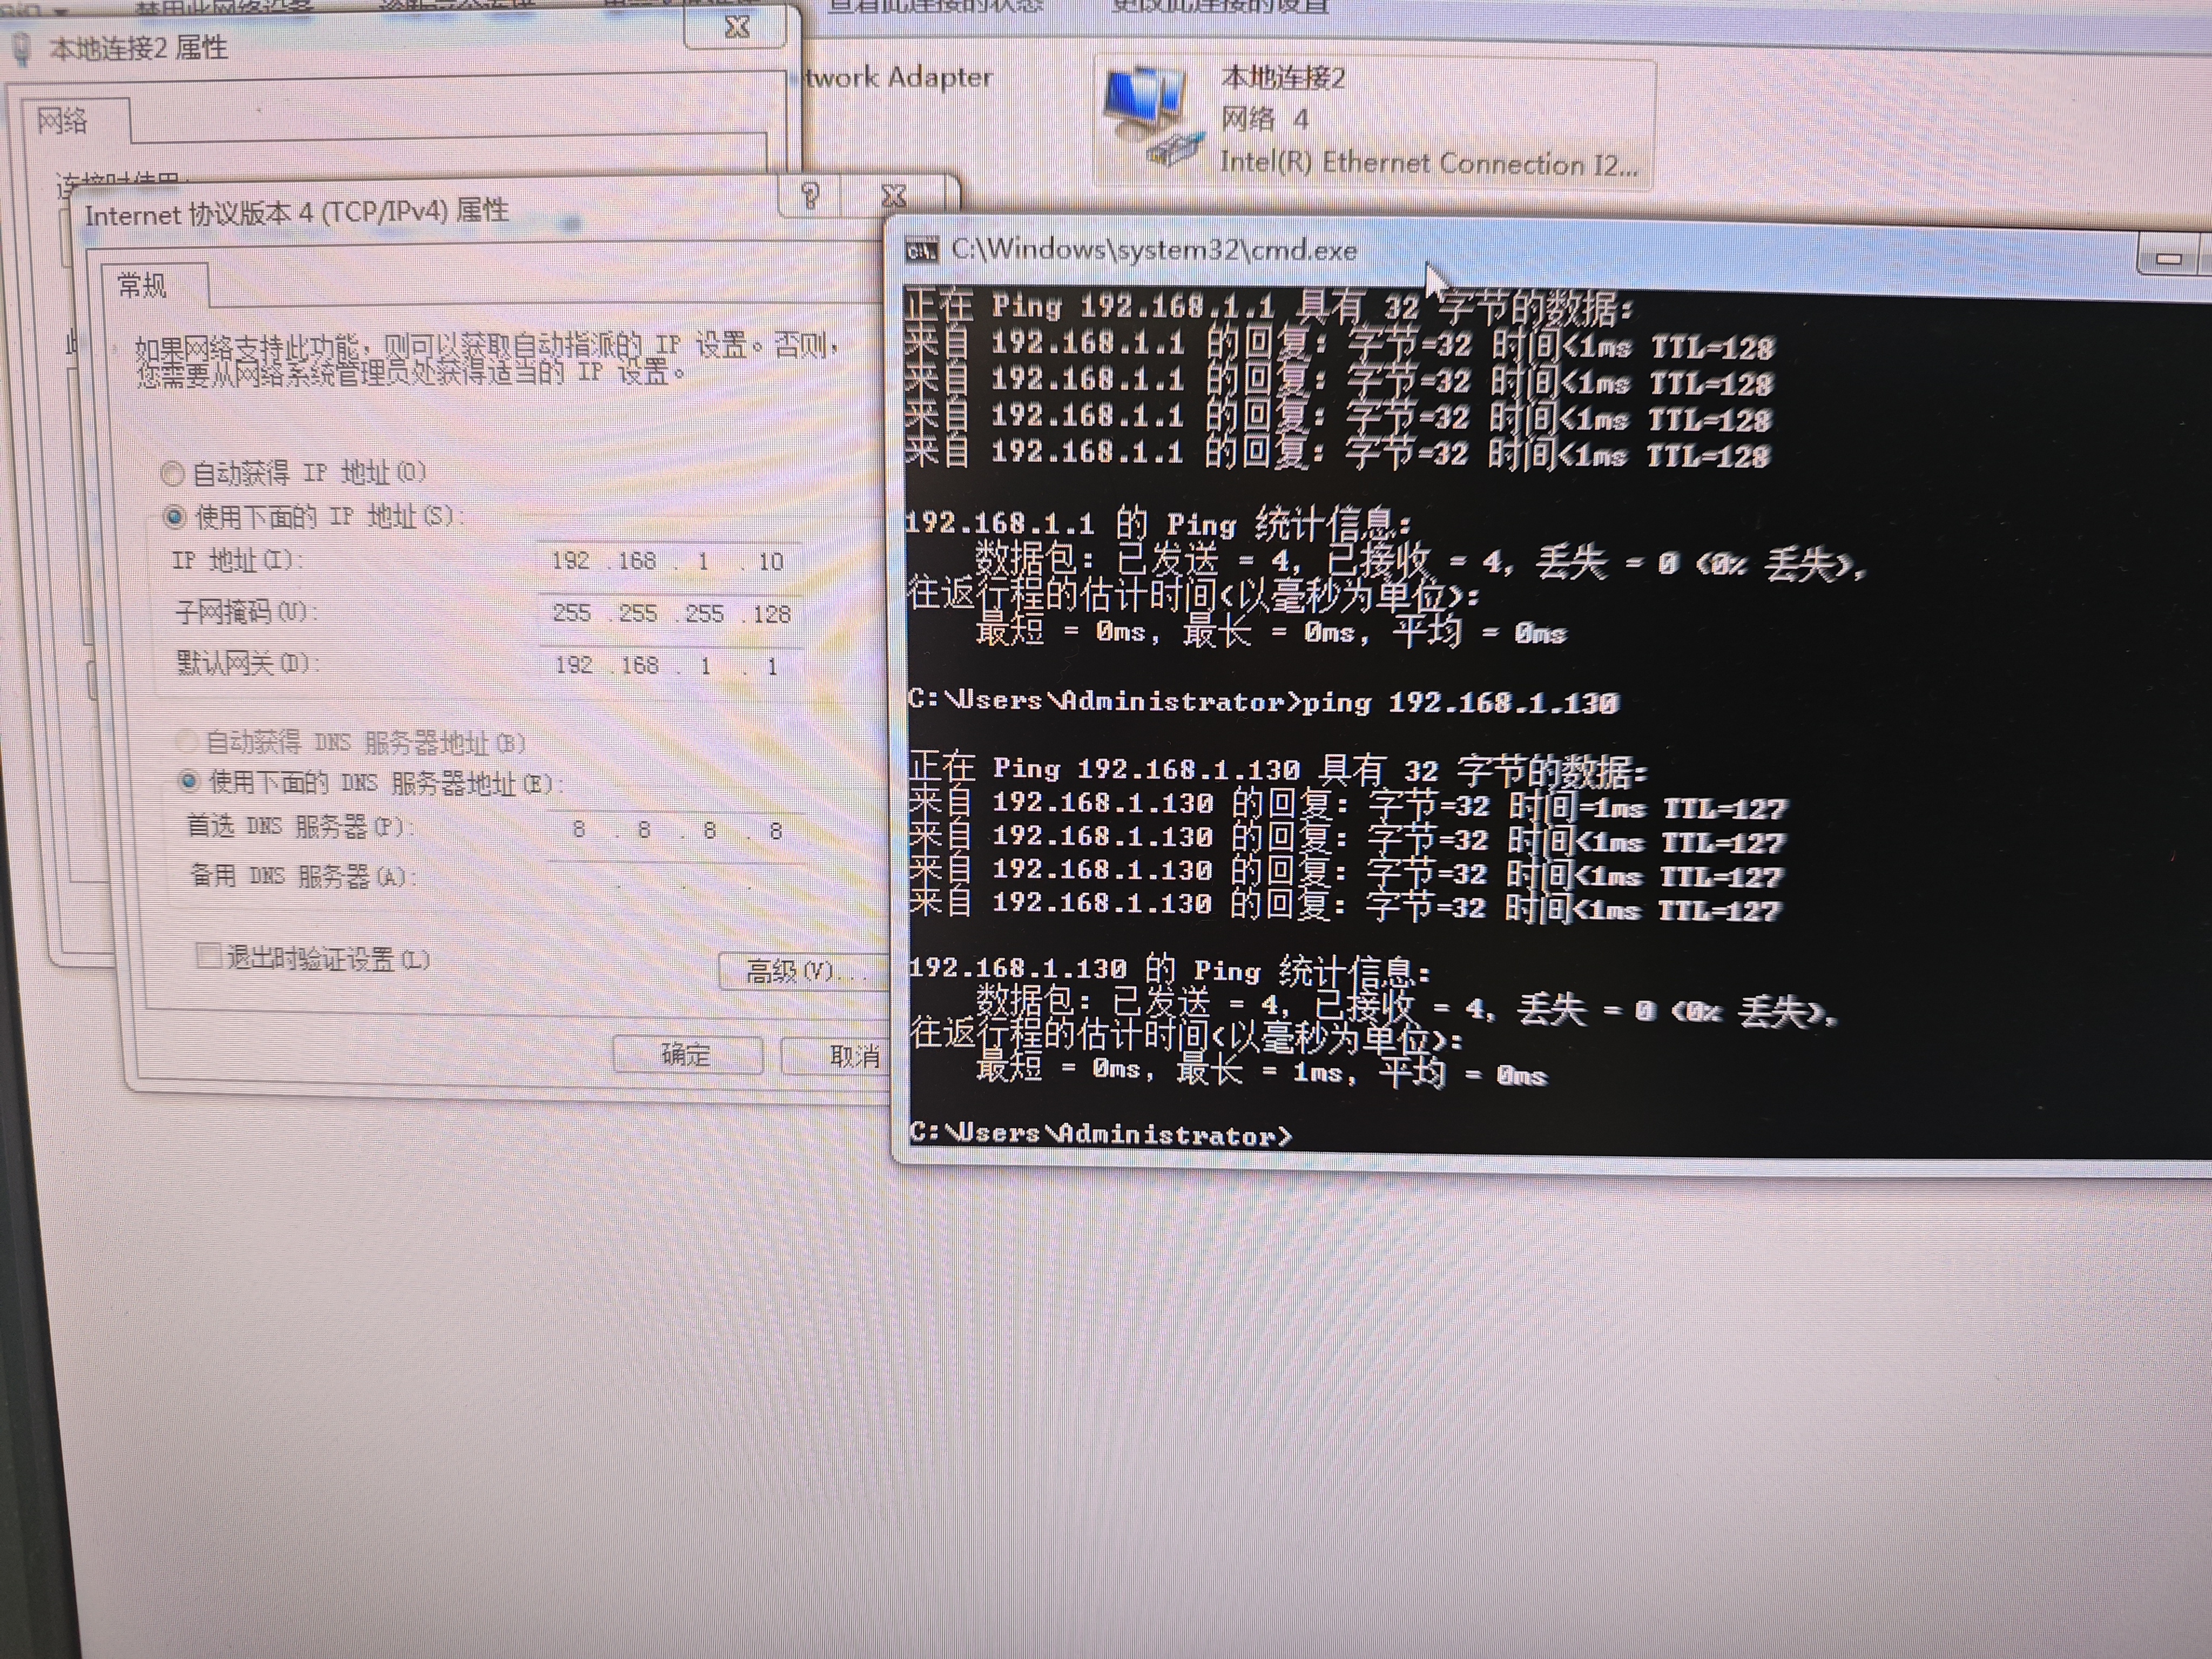
\includegraphics[width=0.8\textwidth]{photo1/image4.jpg}
    \caption{PC1跨子网ping通PC3}
    \label{fig:cross_subnet_ping}
\end{figure}

\newpage
\section{实验二:仿真环境下的互联网组网与路由器配置}

\subsection{实验目标}
使用Cisco Packet Tracer仿真软件,学习路由器的配置方法,并组建一个由多个路由器连接的互联网。通过配置静态路由和动态路由,测试网络的连通性,并观察数据包在网络中的传递过程。

\subsection{实验环境与网络拓扑}
\begin{itemize}
    \item \textbf{仿真软件}: Cisco Packet Tracer
    \item \textbf{网络拓扑}: 3台路由器 (R1, R2, R3),2台交换机,2台PC (PC1, PC2)。拓扑结构如图\ref{fig:sim_topo}所示。
    \item \textbf{子网配置}:
    \begin{itemize}
        \item R1和PC1位于子网 192.168.1.0/24。
        \item R2和PC2位于子网 192.168.2.0/24。
        \item R1与R3通过子网 10.0.0.0/25 连接。
        \item R2与R3通过子网 10.0.1.0/25 连接。
    \end{itemize}
\end{itemize}

\begin{figure}[H]
    \centering
    \includegraphics[width=0.9\textwidth]{photo/image.png}
    \caption{仿真实验网络拓扑}
    \label{fig:sim_topo}
\end{figure}

\subsection{实验步骤(静态路由)}
\begin{enumerate}
    \item 在Packet Tracer中搭建网络拓扑。
    \item 配置R1的端口IP地址。连接交换机的端口IP为192.168.1.1,连接R3的端口IP为10.0.0.1。
    \item 配置R2的端口IP地址。连接交换机的端口IP为192.168.2.1,连接R3的端口IP为10.0.1.2。
    \item 配置R3的端口IP地址。连接R1的端口IP为10.0.0.2,连接R2的端口IP为10.0.1.1。配置完成后如图\ref{fig:r3_ip}所示。
    \item 配置R1的静态路由:告诉R1,要访问192.168.2.0/24网段,下一跳地址是10.0.0.2 (R3的地址)。配置结果如图\ref{fig:r1_route}所示。
    \item 配置R2的静态路由:告诉R2,要访问192.168.1.0/24网段,下一跳地址是10.0.1.1 (R3的地址)。
    \item 配置R3的静态路由:为R3添加到达192.168.1.0/24和192.168.2.0/24两个网段的路由,如图\ref{fig:r3_route}所示。
    \item 配置PC1和PC2的IP地址和默认网关。
\end{enumerate}

\begin{figure}[H]
    \centering
    \includegraphics[width=0.8\textwidth]{photo/image5.png}
    \caption{R3端口IP地址配置结果}
    \label{fig:r3_ip}
\end{figure}

\begin{figure}[H]
    \centering
    \includegraphics[width=0.8\textwidth]{photo/image2.png}
    \caption{R1静态路由配置}
    \label{fig:r1_route}
\end{figure}

\begin{figure}[H]
    \centering
    \includegraphics[width=0.8\textwidth]{photo/image6.png}
    \caption{R3静态路由配置}
    \label{fig:r3_route}
\end{figure}

\subsection{测试结果}
在PC1上ping PC2的IP地址192.168.2.10。如图\ref{fig:sim_ping_result}所示,PC1成功ping通PC2,表明整个网络已经连通,静态路由配置正确。

\begin{figure}[H]
    \centering
    \includegraphics[width=0.8\textwidth]{photo/image1.png}
    \caption{PC1成功ping通PC2}
    \label{fig:sim_ping_result}
\end{figure}

\end{document}
